Schulung der Benutzung von LuftfahrzeugenDie Schulung der Benutzung eines Luftfahrzeuges mittels VR (Virtual-Reality) kann durch einen Flug Simulator mit VR-Funktion angewandt werden.
\begin{figure}[!ht]
    \centering
    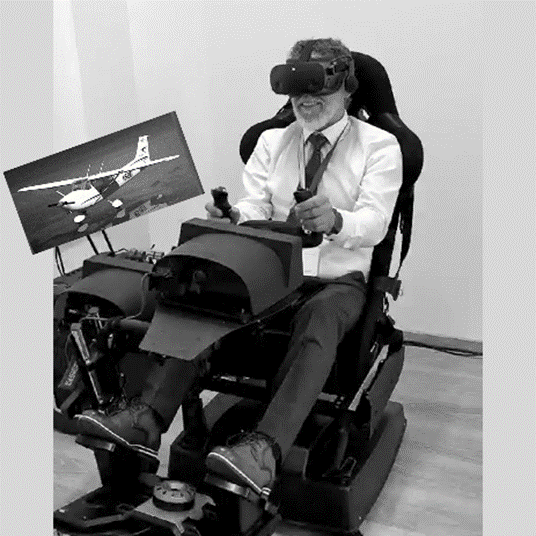
\includegraphics[width=1.0\textwidth]{images/Abbildung 1.png}
    \caption{\label{fig:Abbildung 1}Beispiel für VR-Flugsimulator (Full-motion)\protect
    }
\end{figure}
Dabei ist ein Vorteil des VR-Trainings die Fähigkeit des Simulators eine Welt sehr ähnlich unserer Welt zu replizieren, dadurch können die erlernenden Piloten/Pilotinnen trainieren ohne Schäden und Risiken einzugehen. Jedoch muss bei einem Flug Simulator auch darauf geachtet werden, dass der Simulator den erlernenden Piloten/Pilotinnen auch ein Gefühl des Fliegens vermittelt durch haptisches Feedback zum Beispiel, als Lösung kann ein full-motion Simulator dienen, da dieser auch Bewegung replizieren kann. Das Problem bei diesen full-motion Simulatoren ist, dass diese groß und kostenintensiv sind und deshalb meistens im Besitz von Fluggesellschaften, Leasingunternehmen oder unabhängigen Schulungsorganisationen sind, wodurch diese Simulatoren der Mehrheit der fliegenden Öffentlichkeit nicht zur Verfügung steht. In einer Studie von Ryan Guthridge und Virginia Clinton-Lisell wurden erlernenden Piloten/Pilotinnen in drei Gruppen aufgeteilt wurden, diese Gruppen haben dann jeweils eine andere Trainingsmethode benutzt, dies Methoden sein Computer-software-Training, VR-software-Training und einer Controll-Methode, die kein direktes Training machte sondern nur zuschaute. „In der Nachbefragung, der Studie, beschrieben die Teilnehmer die Vorteile der VR-Technologie als eine praktikable Methode zur Ausbildung von Studentenpiloten. Viele der Antworten waren konsistent und beinhalteten die "Fähigkeit, sich im Flugsimulator um das Flugzeug zu bewegen, indem die Flügel oder andere Objekte als Referenzpunkte verwendet werden". Einige Teilnehmer wiesen darauf hin, dass "VR für Studenten leichter verfügbar und kostengünstiger ist" im Vergleich zu teuren Flugausbildungsgeräten. Schließlich fügten einige Teilnehmer hinzu, dass "VR zu einem vernünftigen Preis für den Heimgebrauch verfügbar ist", was "bei der Vorbereitung auf Lektionen zu Hause vor dem Fliegen des echten Flugzeugs helfen kann". Mit der Weiterentwicklung der Technologie werden Flugschulorganisationen verstärkten Zugang zu kostengünstigen Simulator-alternativen haben. Diese Forschung liefert Beweise, die Pilotenleistungsvariablen sowie qualitative Akzeptanz- und Akzeptanzdaten vergleichen, um VR-Trainingsgeräte und PC-basierte Trainingsgeräte zu bewerten. \cite{guthridge2023evaluating}“ 
Insgesamt hat sich das VR-Training nachweislich positiv auf die Leistung von Studierenden während ihres Ausbildungsverlaufs ausgewirkt. Ganz angekommen ist die VR-Technologie noch nicht, aber wir sind uns ziemlich sicher, dass auch hier die VR-Technologie immer mehr und mehr benutzt werden wird.
Abbildung 1 \footnote{\url{https://legaltech.future-law.at/vr-flug-simulator-auf-der-ltk23/}}
